\chapter{Non-linear SVMs}
\label{cha:non_linear_SVM} Up to this point we have written about linear discriminative
machine learning model. In this section we introduce a non-linear discriminative
model. One of the good properties of SVMs is that they have a theoretically grounded
extension to the non-linear domain.
\newline

Hard-margin SVM can address linearly separable problems. Using these kind of
SVMs we must assume that training data are linearly separable.
\newline

Soft-margin SVM can address linearly separable problems with outliers.
\newline

Non-linearly separable problems need a higher expressive power. These problems are
characterized for example by more complex feature combinations.
\newline

Facing the problem of non-linearly separable problems, we do not want to loose
the advantages of linear separators (i.e. large margin, sparsity of the support vectors,
theoretical guarantees). To achieve these purposes, the solution is to map input
examples (input space) in higher dimensional feature space (this procedure is
called \textit{feature mapping}). Once data are represented in the feature space,
we perform linear classification in this higher dimensional space.

\defi{\textbf{Feature map}\label{def:feature_map}\\ \begin{equation}\Phi : \mathcal{X}\rightarrow \mathcal{H}\end{equation} $\Phi$ is a function mapping each example to a higher dimensional space $\mathcal{H}$ (potentially infinite dimensional). }

Examples $\pmb{x}$ are replaced with their feature mapping $\Phi(\pmb{x})$. The feature
mapping should increase the expressive power of the representation (e.g. introducing
features which are combinations of input features). Examples should be (approximately)
linearly separable in the mapped space.

\section{Example: polynomial mapping}
Sometimes we are interested in considering jointly more variables when building a
predictor on top of them. This can be done with polynomial mapping which maps
features (input vectors) to all possible conjunctions (i.e. products) of features.
There are two types of polynomial mapping:
\begin{enumerate}
	\item \textit{Homogeneous mapping}: maps features to all possible conjunctions
		of features of a certain degree $d$. For example if $d=2$ and we consider
		two features:
		\[
			\Phi(
			\begin{matrix}
				x_{1} \\
				x_{2}
			\end{matrix}) =
			\begin{pmatrix}
				x_{1}^{2}  \\
				x_{1}x_{2} \\
				x_{2}^{2}
			\end{pmatrix}
		\]

	\item \textit{Inhomogeneous mapping}: maps features to all possible conjunctions
		of features up to a certain degree. For example if $d=2$ and we consider two
		features:
		\[
			\Phi(
			\begin{matrix}
				x_{1} \\
				x_{2}
			\end{matrix}) =
			\begin{pmatrix}
				x_{1}      \\
				x_{2}      \\
				x_{1}^{2}  \\
				x_{1}x_{2} \\
				x_{2}^{2}
			\end{pmatrix}
		\]
\end{enumerate}

\textbf{Remark:} the higher the degree, the larger the feature space, the higher
the degree of interactions that we are able to model with the mapping.
\newline

In Figure \ref{fig:example_polinomial_mapping} there is no chance to linearly separate
the examples in the input space. However, if we apply a polynomial ($d=2$) mapping
representing the data in a three dimensional space, examples become linearly
separable.
\newline

\begin{figure}[H]
	\centering
	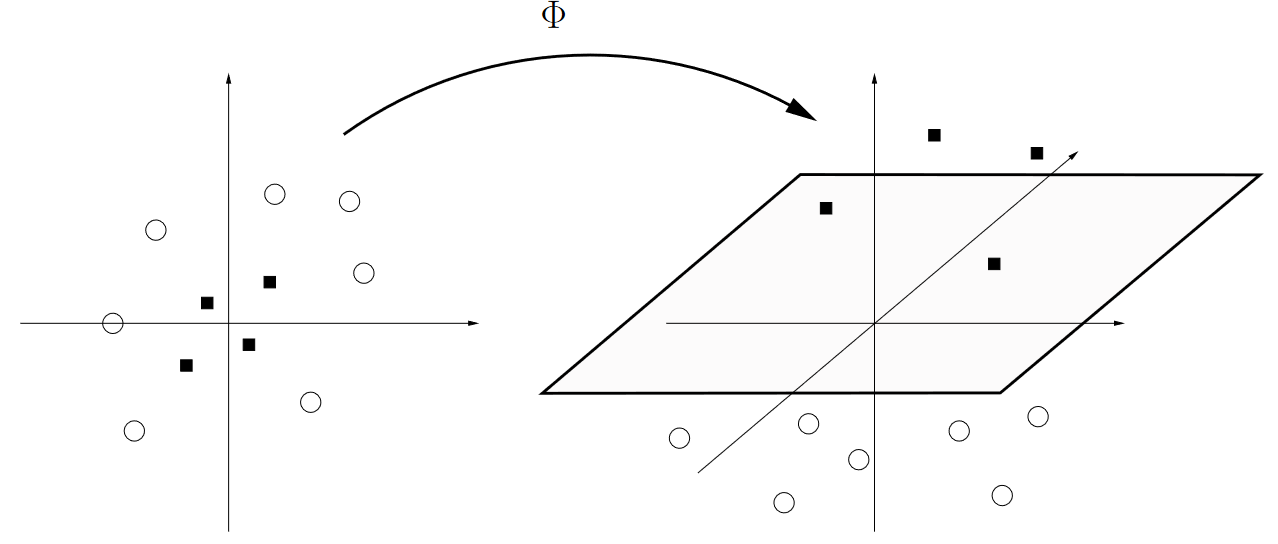
\includegraphics[width=\textwidth]{
		images/14_NonLinearSVMs_polynomialMapping.png
	}
	\caption{If we apply a polynomial mapping representing the data in a three
	dimensional space, examples become linearly separable.}
	\label{fig:example_polinomial_mapping}
\end{figure}

SVM algorithm is applied just replacing $\pmb{x}$ with $\Phi(\pmb{x})$:
\begin{equation}
	f(\pmb{x}) = \pmb{w}^{T}\Phi(\pmb{x}) + w_{0}
\end{equation}

\textbf{Remark:} $\pmb{w}$ in this case is a vector in a three dimensional space.
\newline

A linear separation (i.e. hyperplane) in a feature space corresponds to a non-linear
separation in an input space (Figure \ref{fig:fromHighToLowSpace}) :
\[
	f(
	\begin{matrix}
		x_{1} \\
		x_{2}
	\end{matrix}) = \text{sign}(w_{1}x_{1}^{2}+ w_{2}x_{1}x_{2}+ w_{3}x_{2}^{2}+ w_{0}
	)
\]

Indeed $w_{1}x_{1}^{2}+ w_{2}x_{1}x_{2}+ w_{3}x_{2}^{2}+ w_{0}$ (obtained solving
the dot product between $\pmb{w}^{T}$ and $\Phi(\pmb{x})$) in terms of input
features, is an ellipsoid.
\newline

\begin{figure}[H]
	\centering
	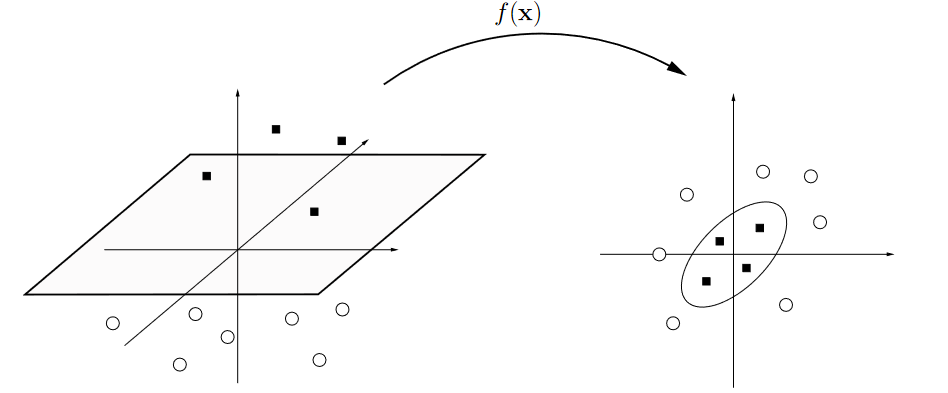
\includegraphics[width=\textwidth]{
		images/14_NonLinearSVMs_fromHighToLowSpace.png
	}
	\caption{A linear separation (i.e. hyperplane) in a feature space corresponds to
	a non-linear separation in an input space.}
	\label{fig:fromHighToLowSpace}
\end{figure}

Once data are mapped in a higher dimensional space, we can apply the same SVM solvers
that we saw in the linearly separable case.

\section{Non-linear SVM in the case of regression}
In the previous chapter we introduced the regularization theory. In that context,
our aim was to combine fitting of the training data, which was measured by means
of weighted penalties, and model complexity which in the classification problem was
the size of the margin.\\ The purpose is the same in the regression case. The
aim is to retain combination of regularization and data fitting (i.e. correctly
approximating the output given the input). Analogously to the classification
case, the result is a trade-off between model complexity (smoothness of the
function) and data fitting. In essence, regularization means smoothness (i.e. smaller
weights, lower complexity) of the learned function. Moreover, the focus is to search
for sparsifying loss to have few support vector. For example, in the previous chapter,
the fact that support vectors were sparse was a consequence of the hinge loss.
\newline

In order to achieve this property in support vector regression, we adopt the $\epsilon$-\textit{intensive
loss}. A commonly used loss function in regression, for example in the deep
learning context, is the square loss ($l(f(\pmb{x}), y) = (f(\pmb{x})-y)^{2}$) or
the mean square error (sum up all the square losses which characterizes all the
training examples and divide by the number of examples) due to its useful properties
(e.g. smoothness). However, if we apply this loss function in the case of SVM we
miss an area where we do not pay anything. The only case when we do not pay anything
is when $f(\pmb{x})$ is exactly equal to $y$, but when dealing with a regression
problem we are considering the continuous domain. The idea is to adopt a loss function
which is more tolerant than this in order to achieve the sparsity property. We
introduce a regression version of the hinge loss which is called $\epsilon$-\textit{intensive
loss} (Figure \ref{fig:insensitive_loss}).

\defi{\textbf{$\epsilon$-insensitive loss}\label{def:eps_insensitive_loss}\\ \begin{equation}\ell (f(\pmb{x}, y)) = |y-f(\pmb{x})|_{\epsilon}= \begin{cases}0&\text{if}|y-f(\pmb{x})| \leq \epsilon \\ |y - f(\pmb{x})| - \epsilon&\text{otherwise}\end{cases}\end{equation} }

\begin{figure}[H]
	\centering
	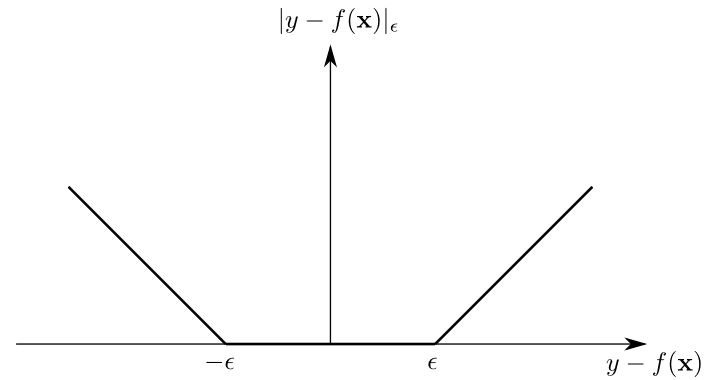
\includegraphics[scale=0.5]{
        images/14_NonLinearSVMs_insensitiveLoss.png
    }
	\caption{The idea is to adopt a loss function which is more tolerant than this
	in order to achieve the sparsity property. We introduce a regression version of
	the hinge loss which is called $\epsilon$-\textit{intensive loss}.}
	\label{fig:insensitive_loss}
\end{figure}

The $\epsilon$-intensive loss depends on the difference between $y$ and
$f(\pmb{x})$ because we are speaking about regression and not classification.
\newline

\textbf{Remark:} in $|y - f(\pmb{x})|_{\epsilon}$, the $\epsilon$ reminds the
positive sign which we have in the hinge loss $|1 - yf(\pmb{x})|_{+}$.
\newline

The result is that we are able to tolerate small ($\epsilon$) deviations from
the true value (i.e. in this tolerance region we pay no penalty). This is
reasonable, remember that in regression the data are typically the result of measurements.
\newline

On the other hand if $|y-f(\pmb{x})|>\epsilon$ we pay a linear penalty as in the
hinge loss. The obtained structure is in some ways a two sided hinge loss.
\newline

In the middle of the function it is defined an $\epsilon$-tube of
insensitiveness around true values. If the difference stays within this tube we do
not pay anything.
\newline

The larger the $\epsilon$ the more tolerant is our model. As well as $C$ in the
linearly separable SVM, also $\epsilon$ is something that we have to configure beforehand
(hyperparameter). Hyperparameters are configured in the model selection stage (basically,
try out different values and evaluate the performance on a validation set).
Playing on $\epsilon$ value allows to trade off function complexity with data
fitting.

\subsection{Support Vector Regression optimization problem}
Let's start with the constraints:
\begin{itemize}
	\item $|y-f(\pmb{x})|_{\epsilon}$ means that for all $i$ it must hold $y_{i}- f
		(\pmb{x_i}) \leq \epsilon$ and $f(\pmb{x_i}) - y_{i}\leq \epsilon$
\end{itemize}

The complexity term is again related to the minimization of the norm of the
weights.
\[
	\text{min}\frac{||w||^{2}}{2}
\]
In the SVM for classification, the complexity term, the norm of the weights,
corresponds to the inverse of the margin. In regression, the norm of the weights
corresponds to the complexity of the function (the number of bumps which we have,
a lot of bumps require a lot of weights).
\newline

With this formulation, we are assuming that all the training examples has to lie
in the $\epsilon$-tube. However, as well as in the case of hard margin SVMs, in order
to be learnable, this formulation could require really large values of
$\epsilon$. As a result, as in the soft margin SVMs, we can introduce slack variables
and penalties for non-satisfied constrains. If we want to relax the condition
$y_{i}- f(\pmb{x_i}) \leq \epsilon$, we can write:
\[
	y_{i}- f(\pmb{x_i}) \leq \epsilon + \xi
\]
and symmetrically:
\[
	f(\pmb{x_i}) - y_{i}\leq \epsilon + \xi^{*}
\]

\textbf{Remark:} we write $\xi^{*}$ in this latter formula to highlight the fact
that $\xi \neq \xi^{*}$.
\newline

Overall, the resulting learning problem is:
\begin{equation}
	\text{min}_{\pmb{w} \in \mathcal{X}, w_0 \in \mathbb{R}, \pmb{\xi}, \pmb{\xi^*}
	\in \mathbb{R}^m}\frac{1}{2}||\pmb{w}||^{2}+ C \sum_{i=1}^{m}(\xi_{i}+ \xi_{i}^{*}
	)
\end{equation}
subject to
\[
	\pmb{w}^{T}\Phi(\pmb{x_i}) + w_{0}- y_{i}\leq \epsilon + \xi_{i}
\]
\[
	y_{i}- (\pmb{w}^{T}\Phi(\pmb{x_i})+w_{0}) \leq \epsilon + \xi_{i}^{*}
\]
\[
	\xi_{i}, \xi_{i}^{*}\geq 0
\]

\textbf{Remark:} we get two constraints for each example for the upper and lower
sides of the tube. Slack variables $\xi_{i}$, $\xi_{j}^{*}$ penalize predictions
out of the $\epsilon$-insensitive tube.
\newline

\textbf{Remark:} again the obtained formula is a quadratic optimization problem
with linear constraints.

\subsection{Lagrangian in the regression case}
As well as in the classification case, we can address the regression optimization
problem using Lagrange multipliers. We include constraints in the minimization
function using Lagrange multipliers ($\alpha_{i}, \alpha_{i}^{*}, \beta_{i}, \beta
_{i}^{*}, \beta_{i}^{*}\geq 0$).

\begin{itemize}
	\item \textbf{constraint 1:}
		\[
			f(\pmb{x_i})-y_{i}\leq \epsilon + \xi_{i}
		\]
		\[
			\epsilon + \xi_{i}-f(\pmb{x_i})+y_{i}\geq 0
		\]

	\item \textbf{constraint 2:}
		\[
			y_{i}- f(\pmb{x_i}) \leq \epsilon + \xi_{i}
		\]
		\[
			\epsilon + \xi_{i}-y_{i}+ f(\pmb{x_i}) \geq 0
		\]

	\item \textbf{constraint 3:}
		\[
			\xi_{i}\geq 0
		\]

	\item \textbf{constraint 4:}
		\[
			\xi_{i}^{*}\geq 0
		\]
\end{itemize}

The Lagrangian is:
\begin{align*}
	L = \frac{||\pmb{w}||^{2}}{2}+ C \sum_{i}(\xi_{i}+ \xi_{i}^{*})      &  \\
	- \sum_{i}\alpha_{i}(\epsilon + \xi_{i}- y_{i}+ f(\pmb{x_i}))        &  \\
	- \sum_{i}\alpha_{i}^{*}(\epsilon + \xi_{i}^{*}- f(\pmb{x_i})+y_{i}) &  \\
	- \sum_{i}\beta_{i}\xi_{i}                                           &  \\
	- \sum_{i}\beta_{i}^{*}\xi_{i}^{*}
\end{align*}

In this case the primal variables are: $\pmb{w}$, $w_{0}$, $\pmb{\xi}$, $\pmb{\xi}
^{*}$.

I compute the gradient of the Lagrangian with respect to $\pmb{w}$. Some terms
disappear because they do not depend on $\pmb{w}$.

\[
	\nabla_{\pmb{w}}L = \pmb{w}- \nabla_{\pmb{w}}\sum_{i}\alpha_{i}(\pmb{w}^{T}\Phi
	(\pmb{x_i}) + w_{0}) + \nabla_{\pmb{w}}\sum_{i}\alpha_{i}^{*}(\pmb{w}^{T}\Phi (
	\pmb{x_i}) + w_{0}) =
\]
\[
	\pmb{w}- \sum_{i}\alpha_{i}\Phi(\pmb{x_i}) + \sum_{i}\alpha_{i}^{*}\Phi(\pmb{x_i}
	)
\]

We now vanish the gradient setting it to zero.

\[
	\nabla_{\pmb{w}}L = \pmb{w}- \sum_{i}\alpha_{i}\Phi(\pmb{x_i}) + \sum_{i}\alpha
	_{i}^{*}\Phi(\pmb{x_i}) = 0
\]

\[
	\pmb{w}= \sum_{i}(\alpha_{i}-\alpha_{i}^{*}) \Phi(\pmb{x_i})
\]

Again $\pmb{w}$ is a linear combination of training examples with coefficients $(
\alpha_{i}- \alpha_{i}^{*})$.
\newline

Now we compute the derivative of the Lagrange with respect to $w_{0}$.
\[
	\frac{\partial L}{\partial w_{0}}= \frac{\partial}{\partial w_{0}}- \sum_{i}\alpha
	_{i}(w_{0}) + \frac{\partial}{\partial w_{0}}\sum_{i}\alpha_{i}^{*}(w_{0})
\]

Setting this latter result equal to zero we get:
\[
	\frac{\partial L}{\partial w_{0}}= - \sum_{i}\alpha_{i}+ \sum_{i}\alpha_{i}^{*}
	= 0
\]
\[
	\sum_{i}(\alpha_{i}^{*}- \alpha_{i}) = 0
\]

The result is a constraint on the sum of the alphas.
\newline

Now we compute the derivative with respect to $\pmb{\xi}$.

\[
	\frac{\partial L}{\partial \xi_{i}}= \frac{\partial }{\partial \xi_{i}}(C \xi_{i}
	- \alpha_{i}\xi_{i}- \beta_{i}\xi_{i})
\]

If we set this equal to zero we obtain the same result as in the classification
case:
\[
	C - \alpha_{i}- \beta_{i}= 0
\]
\newline

The derivative with respect to $\pmb{\xi}^{*}$ is the more or less the same.
\[
	\frac{\partial L}{\partial \xi_{i}^{*}}= C - \alpha_{i}^{*}- \beta_{i}^{*}= 0
\]

At this point we have to replace the obtained result in the Lagrangian.
\newline

First of all we think about $\pmb{w}$ highlighting where it appears:
\[
	\frac{\pmb{w}^{T}\pmb{w}}{2}- \sum_{i}\alpha_{i}\pmb{w}^{T}\Phi(\pmb{x_i}) + \sum
	_{i}\alpha_{i}^{*}\pmb{w}^{T}\Phi(x_{i})
\]

Now we replace $\pmb{w}$ with the expression discovered above.
\[
	(\frac{1}{2}\sum_{i}(\alpha_{i}- \alpha_{i}^{*}) \Phi(x_{i}))^{T}(\sum_{j}( \alpha
	_{j}- \alpha_{j}^{*}) \Phi(x_{j})) - \sum_{i}(\alpha_{i}- \alpha_{i}^{*}) (\sum
	_{j}(\alpha_{j}- \alpha_{j}^{*}) \Phi(x_{j}))^{T}\Phi(x_{i})
\]

This expression contains two pieces which are the same only one is twice with
respect to the other:
\[
	(\frac{1}{2}\sum_{i}(\alpha_{i}- \alpha_{i}^{*}) \Phi(x_{i}))^{T}(\sum_{j}( \alpha
	_{j}- \alpha_{j}^{*}) \Phi(x_{j})) - \sum_{i}(\alpha_{i}- \alpha_{i}^{*}) (\sum
	_{j}(\alpha_{j}- \alpha_{j}^{*}) \Phi(x_{j}))^{T}\Phi(x_{i}) =
\]
\[
	-\frac{1}{2}\sum_{i}\sum_{j}(\alpha_{i}- \alpha_{i}^{*}) (\alpha_{j}- \alpha_{j}
	^{*}) \Phi(x_{i})^{T}\Phi(x_{j})
\]

The obtained result is really similar to the one obtained in the classification
case.
\newline

Now we do the same thing for $w_{0}$. First of all we highlight where it appears:
\[
	- \sum_{i}\alpha_{i}w_{0}+ \sum_{i}\alpha_{i}^{*}w_{0}= w_{0}\sum_{i}(\alpha_{i}
	^{*}- \alpha_{i})
\]
Since $\sum_{i}(\alpha_{i}^{*}- \alpha_{i}) = 0$ we get:
\[
	w_{0}\sum_{i}(\alpha_{i}^{*}- \alpha_{i}) = 0
\]

Then we examine the component with $\xi_{i}$.
\[
	\sum_{i}\xi_{i}(C - \alpha_{i}- \beta_{i}) = 0
\]

The same holds for $\xi_{i}^{*}$.
\[
	\sum_{i}\xi_{i}^{*}(C - \alpha_{i}^{*}- \beta_{i}^{*}) = 0
\]

We now consider the pieces where $\epsilon$ appears:
\[
	- \sum_{i}\alpha_{i}\epsilon - \sum_{i}\alpha_{i}^{*}\epsilon + \sum_{i}\alpha_{i}
	y_{i}- \sum_{i}\alpha_{i}^{*}y_{i}
\]

At the end of the day we get the dual formulation:

\[
	\begin{array}{cl}
		\max _{\boldsymbol{\alpha} \in \mathbb{R}^m} & -\frac{1}{2} \sum_{i, j=1}^m\left(\alpha_i^*-\alpha_i\right)\left(\alpha_j^*-\alpha_j\right) \Phi\left(\mathbf{x}_i\right)^T \Phi\left(\mathbf{x}_j\right) \\
		\\
		                                             & -\epsilon \sum_{i=1}^m\left(\alpha_i^*+\alpha_i\right)+\sum_{i=1}^m y_i\left(\alpha_i^*-\alpha_i\right)                                                    \\
		\\
		\text{ subject to }                          & \sum_{i=1}^m\left(\alpha_i-\alpha_i^*\right)=0                                                                                                             \\
		\\
		                                             & \alpha_i, \alpha_i^* \in[0, C] \quad \forall i \in[1, m]
	\end{array}
\]

$\alpha_{i}, \alpha_{i}^{*}\in [0,C]$ because of $C - \alpha_{i}- \beta_{i}= 0$ and
$C - \alpha_{i}^{*}- \beta_{i}= 0$
\newline

As well as in the classification case, the obtained result is still a quadratic optimization
problem with box constraints.
\newline

It we replace $\pmb{w}$ in the decision function with its dual formulation $\pmb{w}
= \sum_{i}(\alpha_{i}-\alpha_{i}^{*}) \Phi(\pmb{x_i})$ we get:
\[
	f(\pmb{x}) = \pmb{w}^{T}\Phi(\pmb{x}) + w_{0}= \sum_{i=1}^{m}(\alpha_{i}- \alpha
	_{i}^{*}) \Phi(\pmb{x_i})^{T}\Phi(\pmb{x}) + w_{0}
\]

\textbf{Remark:} if $\Phi$ is the identity function then this is linear
regression. So, we can do linear regression with SVM. If $\Phi$ is not the identity
function we are doing non linear regression.

\subsection{Karush-Khun-Tucker conditions (KKT) in the case of support vector
regression}
In this subsection we reason about the support vectors properties in the dual formulation
which we have just introduced. The KKT conditions requires that all terms where
the Lagrange multipliers appear should be equal to zero. So, at the saddle point
it holds that for all $i$:
\[
	\alpha_{i}(\epsilon + \xi_{i}+ y_{i}- \pmb{w}^{T}\Phi(\pmb{x_i}) - w_{0}) = 0
\]
\[
	\alpha_{i}^{*}(\epsilon + \xi_{i}^{*}- y_{i}+ \pmb{w}^{T}\Phi(\pmb{x_i}) + w_{0}
	) = 0
\]
\[
	\beta_{i}\xi_{i}= 0
\]
\[
	\beta_{i}^{*}\xi_{i}^{*}= 0
\]

Combined with $C - \alpha_{i}- \beta_{i}= 0$, $\alpha_{i}\geq 0$,
$\beta_{i}\geq 0$ and $C - \alpha_{i}^{*}- \beta_{i}^{*}= 0$, $\alpha_{i}^{*}\geq
0$, $\beta_{i}^{*}\geq 0$ we get:
\[
	\alpha_{i}\in [0,C]
\]
\[
	\alpha_{i}^{*}\in [0,C]
\]
and
\[
	\alpha_{i}= C \quad \text{ if }\xi_{i}> 0
\]
\[
	\alpha_{i}^{*}= C \quad \text{ if }\xi_{i}^{*}> 0
\]

Notice that in
$f(\pmb{x}) = \sum_{i=1}^{m}(\alpha_{i}- \alpha_{i}^{*}) \Phi(\pmb{x_i})^{T}\Phi
(\pmb{x}) + w_{0}$
in order for an example to not be a support vector both $\alpha_{i}$ and
$\alpha_{i}^{*}$ must be zero. Indeed, an example could be over the tube or
below the tube and not satisfy the constraints. To satisfy the constraint the example
should be inside the tube. If this is not the case, only one of the two alphas can
be non zero because the example cannot be over and below the tube at the same time.
\newline
If for example $\alpha_{i}\neq 0$ then
$(\epsilon + \xi_{i}+ y_{i}- \pmb{w}^{T}\Phi(\pmb{x_i}) - w_{0}) = 0$.\\ If also
$\xi_{i}= 0$, than it means that the difference between $f(\pmb{x_i})$ and $y_{i}$
is exactly $\epsilon$. In this case there is no penalty because we are on the
boundary of the tube.\\If instead $\xi_{i}> 0$ the difference between $y_{i}$ and
$f(\pmb{x_i})$ is larger than $\epsilon$. In this case $\beta_{i}= 0$ and so
$\alpha_{i}= C$.\\ The same reasoning works symmetrically for the $*$ case.
\newline

\textbf{Remark:} according to the professor $\alpha_{i}\in [0,C]$ is not only a consequence
of $C - \alpha_{i}- \beta_{i}= 0$, $\alpha_{i}\geq 0$, $\beta_{i}\geq 0$, but
also of $\beta_{i}\xi_{i}= 0$. At this moment, the author is not convinced about
this claim. Maybe in the future I will understand.
\newline

We can sum up the obtained results as follows:
\begin{itemize}
	\item All patterns within the $\epsilon$-tube, for which
		$|f(\pmb{x_i})-y_{i}| < \epsilon$, have $\alpha_{i}, \alpha_{i}^{*}= 0$ and thus
		don't contribute to the estimated function $f$. All the examples which lie
		inside the tube are not support vectors.

	\item Patterns for which either $0 < \alpha_{i}< C$ or $0 < \alpha_{i}^{*}< C$
		(they cannot be both non-zero at the same time) are on the border of the $\epsilon$-tube,
		that is $|f(\pmb{x_i})-y_{i}| = \epsilon$. They are the unbound support vectors.
		(It is like staying exactly on the confidence one hyperplane).

	\item The remaining training patterns are margin errors (either $\xi_{i}> 0$
		or $\xi_{i}^{*}> 0$), and reside out of the $\epsilon$-insensitive region. They
		are bound support vectors, with corresponding $\alpha_{i}= C$ or
		$\alpha_{i}^{*}= C$.
\end{itemize}

For the sake of clarity, Figure \ref{fig:svm_regression_graphically} illustrates
the concept graphically.

\begin{figure}[H]
	\centering
	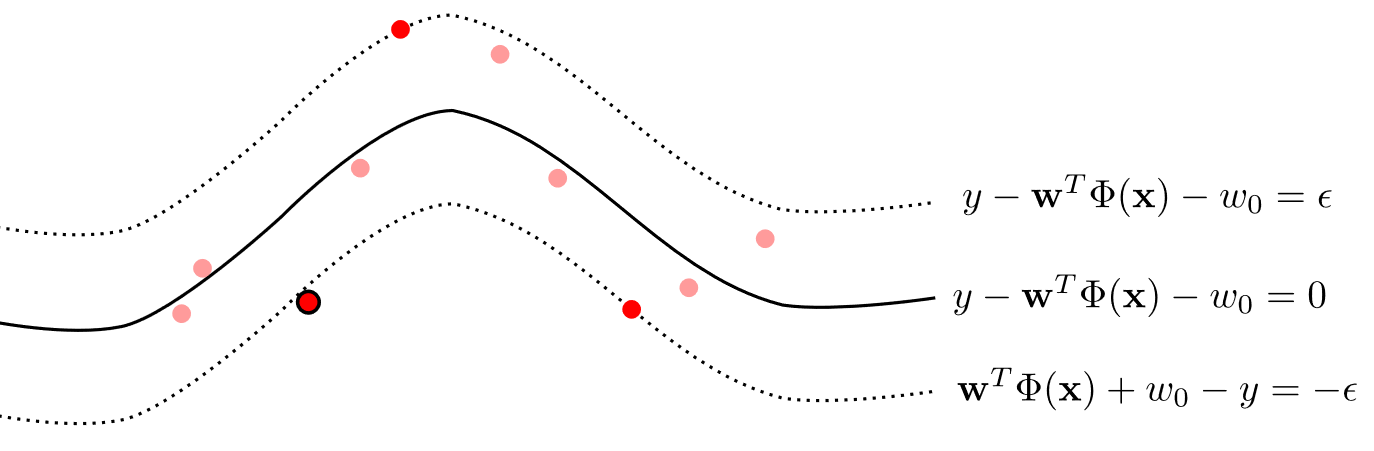
\includegraphics[width=\textwidth]{
		images/14_NonLinearSVMs_regressionGraphically.png
	}
	\caption{The solid curve corresponds to the regions where
	$y - \pmb{w}^{T}\Phi{\pmb{x}}- w_{0}= 0$. The two parallel curves are where $y
	- \pmb{w}^{T}\Phi{\pmb{x}}- w_{0}= \epsilon$ and $\pmb{w}^{T}\Phi{\pmb{x}}- w_{0}
	- y = - \epsilon$.}
	\label{fig:svm_regression_graphically}
\end{figure}

The solid curve corresponds to the regions where $y - \pmb{w}^{T}\Phi{\pmb{x}}- w
_{0}= 0$. The two parallel curves are where
$y - \pmb{w}^{T}\Phi{\pmb{x}}- w_{0}= \epsilon$ and
$\pmb{w}^{T}\Phi{\pmb{x}}- w_{0}- y = - \epsilon$. The space between the two parallel
curves with the solid curve in the middle is the $\epsilon$-insensitive tube.
This structure reminds the classification case. In this last, examples must be
outside the margin. In this case we look for examples which stay inside the tube.\\
All the shaded points, which correspond to the points inside the tube, are not support
vectors. \\ The examples which stay exactly on the border of the tube are
unbound support vectors. \\ The red point which is slightly out of the tube is a
bound support vector.
\newline

Looking at Figure \ref{fig:svm_regression_decreasing_eps} we notice that reducing
$\epsilon$ the tube becomes smaller. The function can accommodate more bumps if
needed (it has more flexibility). As a result the number of support vector increases.
Indeed, if the tube becomes smaller it is difficult that examples stay inside the
tube. In the third case the tube is really small, as a result almost all the points
are support vectors. \\ In conclusion we understood that the complexity of the
function is regulated by the minimization of the weights and by the
configuration of the hyperparameter $\epsilon$ which corresponds to the size of
the tube.
\newline

\textbf{Remark:} in the last case of Figure \ref{fig:svm_regression_decreasing_eps}
it is clear that we are allowing too much flexibility. In this case we tend to
interpolate all the examples including their noise.

\begin{figure}[H]
	\centering
	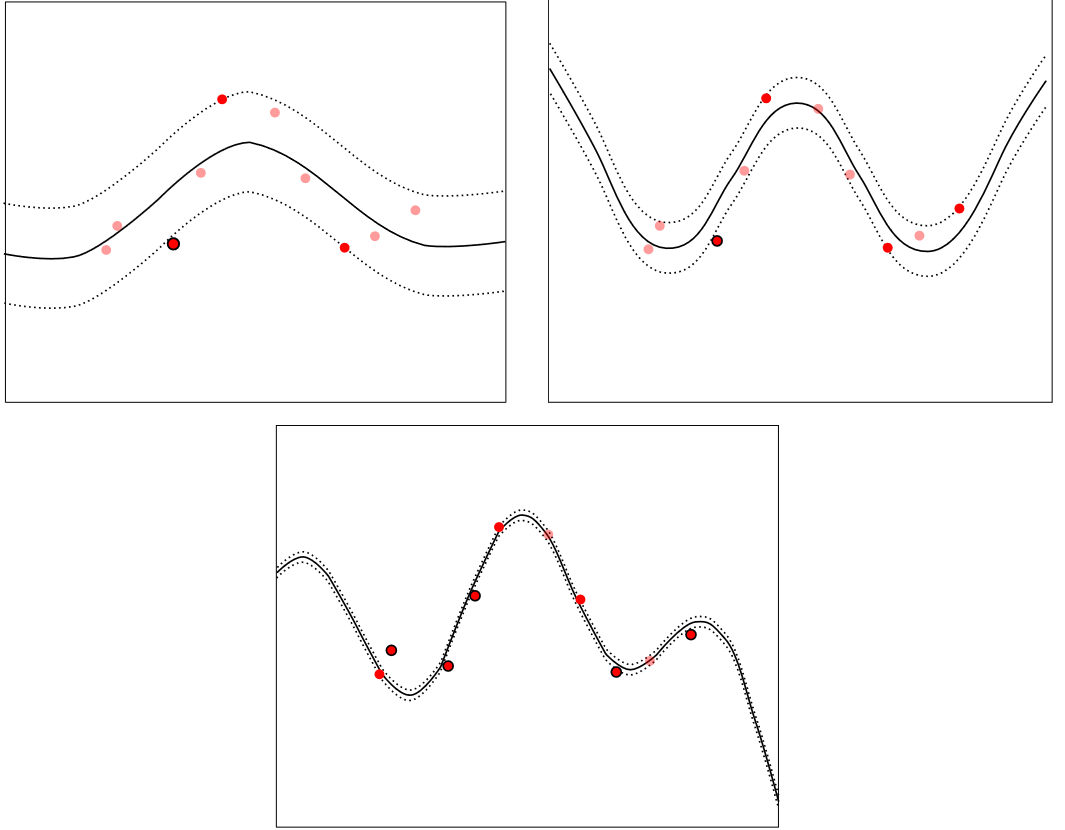
\includegraphics[width=0.85\textwidth]{
		images/14_NonLinearSVMs_regressionEpsilonValues.png
	}
	\caption{Reducing $\epsilon$, the size of the tube reduces.}
	\label{fig:svm_regression_decreasing_eps}
\end{figure}